\chapter{Przykłady wykorzystania systemu}

Aplikacja RevCommnunity posiada szereg zaimplementowanych funkcjonalności. Należą do nich między innymi:

\begin{itemize}
\item Rejestracja nowego użytkownika w~systemie
\item Dodawanie nowego produktu i~umieszczanie go w~wybranej kategorii, dostępnej w~systemie
\item Definiowanie nowej kategorii oraz umieszczanie jej na odpowiednim miejscu w~drzewie kategorii
\item Tworzenie recenzji dla konkretnego produktu
\item Przeglądanie najnowszych produktów oraz recenzji z~możliwością ich filtrowania
\item Przeglądanie drzewa kategorii, filtrowanie produktów względem kategorii oraz wyszukiwanie produktów
\item Import danych z~zewnętrznych serwisów
\end{itemize}

\section{Rejestracja nowego użytkownika w~systemie}

Rejestracja nowego użytkownika jest możliwa po wypełnieniu formularza oraz zatwierdzeniu wprowadzonych danych, poprzez wciśnięcie przycisku „Zarejestruj się”.

Formularz umożliwiający rejestrację nowego użytkownika jest walidowany w~czasie rzeczywisty co oznacza, że po każdej akcji wykonanej na formularzu przez użytkownika, następuje sprawdzenie czy wartości wpisane w~poszczególnych polach są prawidłowe.

\begin{figure}[h]
	\centering
	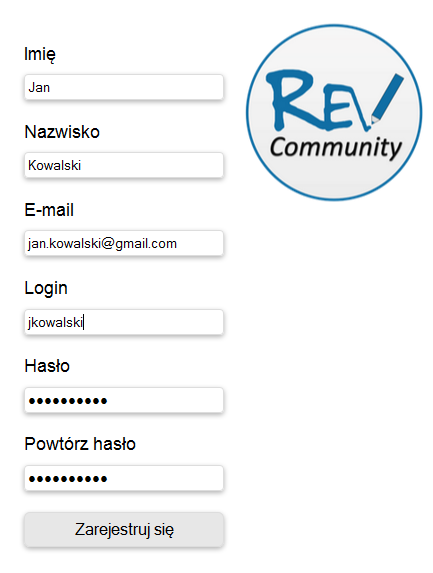
\includegraphics[scale=0.6]{images/rejestracja.png}
	\caption{Wypełniony formularz rejestracji nowego użytkownika.}
\end{figure}

\begin{figure}[h]
	\centering
	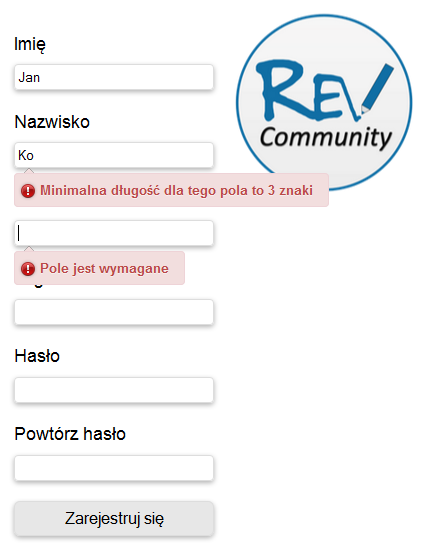
\includegraphics[scale=0.6]{images/rejestracja_walidacja.png}
	\caption{Formularz z~błędnie wypłnionymi polami.}
\end{figure}

\newpage
\section{Dodawanie nowego produktu}

Ekran ten umożliwia dodanie nowego produktu w~systemie. Produkt można opisać podstawowymi metadanymi w~panelu „Specyfikacja” oraz przypisać go do kategorii w~ramach sekcji „Wybór kategorii”. Przy pomocy rozbudowanego edytora HTML, istnieje możliwość stworzenia profesjonalnego opisu produktu. W opisie można również umieścić obrazy oraz filmy.

\begin{figure}[h]
	\centering
	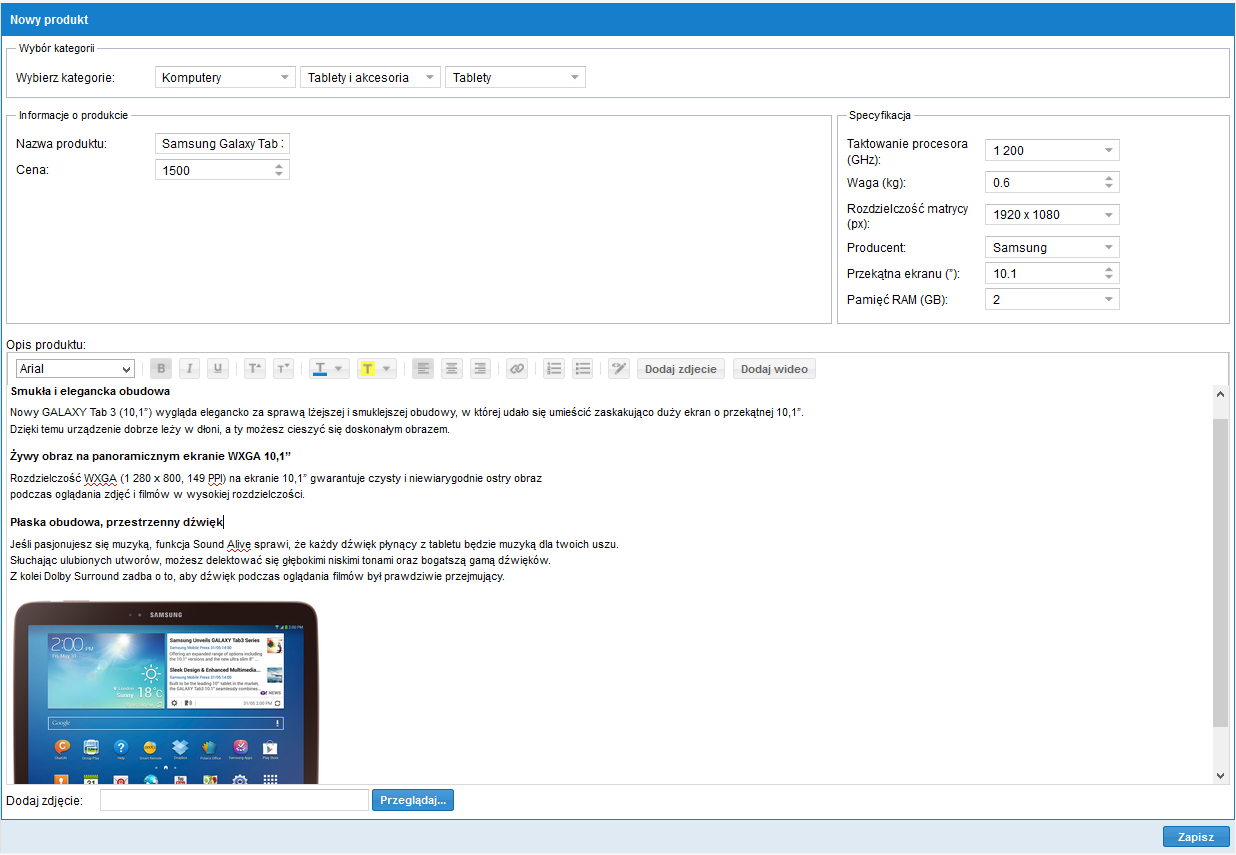
\includegraphics[width=1.00\textwidth]{images/nowy_produkt.PNG}
	\caption{Widok dodawania nowego produktu.}
\end{figure}

\section{Definiowanie nowej kategorii}

W ekranie tworzenia nowej kategorii mamy możliwość stworzenia zarówno kategorii pośredniej jak i~końcowej. Definiując kategorię wybieramy ścieżkę w~drzewie, które odpowiada miejscu umieszczenia kategorii. W przypadku gdy kategoria jest kategorią końcową, istnieje możliwość dodania parametrów opisujących produkty, które do niej należą.Parametr definiowany jest poprzez nazwę oraz typ wartości. Dostępnymi typami są:
\begin{itemize}
\item Tekst
\item Lista
\item Data
\item Liczba
\end{itemize}
W przypadku typu „Lista”, należy dodatkowo podać wartości, które mają się na niej znajdować. Wartości  możemy dodać po kliknięci przycisku „Dodaj Wartość”.

\begin{figure}[h]
	\centering
	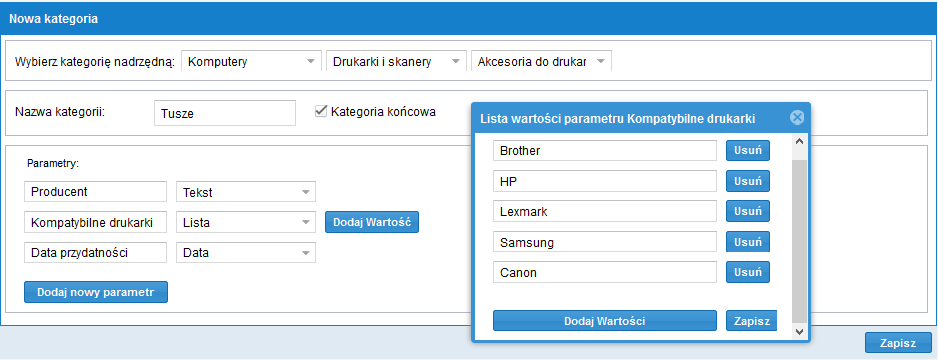
\includegraphics[width=1.00\textwidth]{images/nowa_kategoria.PNG}
	\caption{Widok dodawania nowej kategorii.}
\end{figure}
% Musiałem dodac znacznik newpage poniewaz zdjecie uciekalo
\newpage

\section{Tworzenie recenzji dla konkretnego produktu}

Tworzenie nowej recenzji polega na ocenieniu produktu w~skali od 0-5 oraz stworzeniu opisu będącego opinią na jego temat. Dzięki rozbudowanemu edytorowi HTML, możliwe jest tworzenie profesjonalnego opisu, zawierającego obrazy oraz filmy. Po kliknięciu przycisku „Zapisz”, recenzja będzie widoczna przez pozostałych użytkowników RevCommunity. Od tego momentu możliwe jest ocenianie tej recenzji, a~tym samym kształtowanie wizerunku jej autora.

\begin{figure}[h]
	\centering
	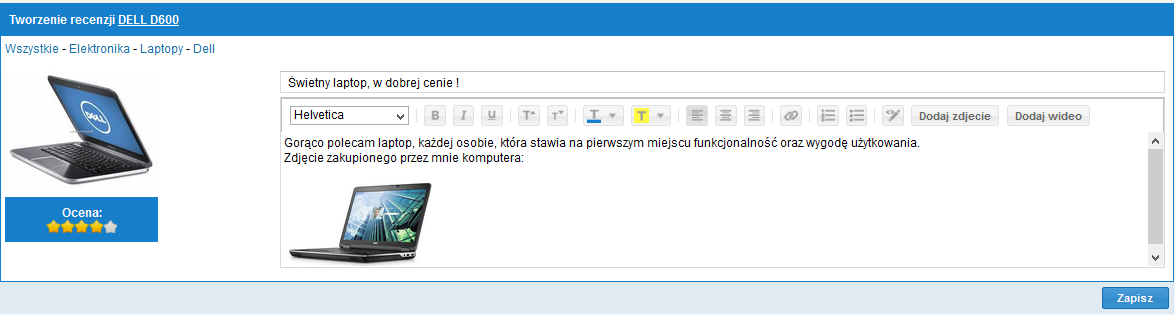
\includegraphics[width=1.00\textwidth]{images/nowa_recenzja.PNG}
	\caption{Widok dodawania nowej recenzji.}
\end{figure}

\section{Panel główny}

\subsection{Przeglądanie najnowszych produktów oraz recenzji}

W panelu głównym użytkownik ma możliwość wykonać następujące akcje:

\begin{itemize}
\item Wyszukać produkty
\item Posortować oraz przefiltrować produkty
\item Posortować recenzje
\end{itemize}

Sortowanie produktów i~recenzji odbywa się poprzez wybranie parametru po którym sortowanie ma się odbyć oraz poprzez wybranie kierunku sortowania, rosnącego lub malejącego.

\subsection{Przeglądanie drzewa kategorii}

W panelu nawigacyjnym użytkownik ma możliwość przeglądania drzewa kategorii oraz wyszukiwania produktów. Po kliknięciu na znak „+” lub „-”, znajdujący się po lewej stronie nazwy kategorii, następuje rozwinięcie lub zwinięcie drzewa z~kategoriami. W ten sposób użytkownik może wygodnie nawigować po wszystkich kategoriach dostępnych w~systemie. Po kliknięciu na nazwę kategorii, następuje nałożenie filtru. Od tej pory, widoczne są jedynie produkty w~ramach tej kategorii oraz kategorii podrzędnych.

\begin{figure}[h]
	\centering
	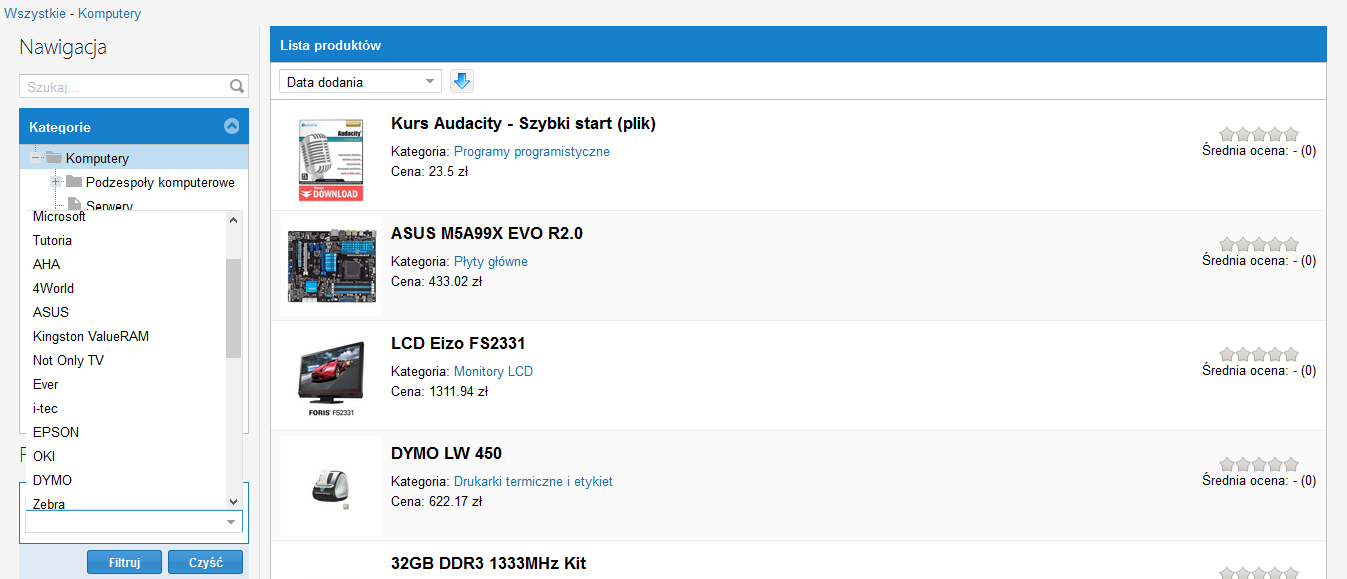
\includegraphics[width=1.00\textwidth]{images/filtr_kategorii.png}
	\caption{Widok produktów z~kategorii "Komputery"}
\end{figure}

W panelu nawigacyjnym, użytkownik ma również możliwość filtrowania produktów po parametrach opisujących produkty w~danej kategorii. Na powyższym rysunku istnieje możliwość filtrowania produktów po nazwie producenta w~ramach kategorii komputery.
\paragraph{}
Po przeprowadzeniu operacji filtrowania u góry ekranu pojawi się pasek przypominający użytkownikowi o~filtrze, który zastosował. Wciśnięcie ikony z~literą „x” na pomarańczowym tle, spowoduje usunięcie filtru i~ponowne przedstawienie wszystkich produktów w~ramach kategorii „Komputery”.

\begin{figure}[h]
	\centering
	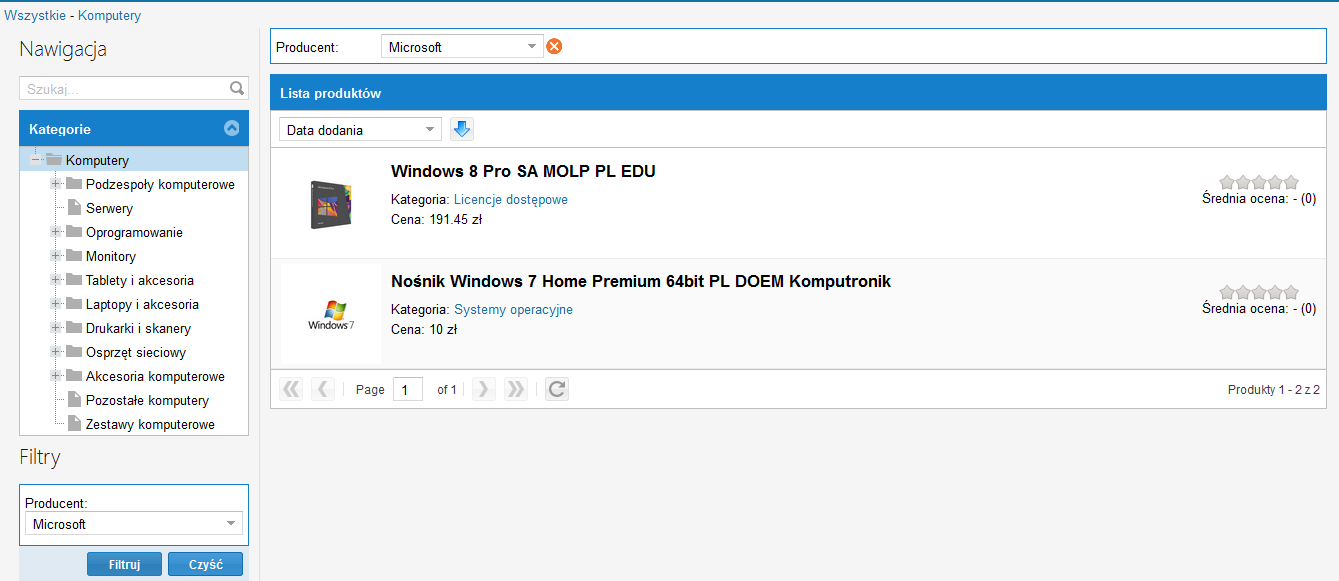
\includegraphics[width=1.00\textwidth]{images/po_nalozeniu_filtru_kategoria.png}
	\caption{Widok przefiltrowanych produktów po nazwie producenta.}
\end{figure}

\newpage

U góry panelu nawigacyjnego znajduje się również wyszukiwarka. Umożliwia ona wyszukiwanie pełno tekstowe, dzięki temu szukana fraza może dotyczyć:

\begin{itemize}
\item Nazwy produktu
\item Wartości parametrów powiązanych z~produktem
\item Fragmentu opisu produktu
\end{itemize}

\section{Import danych z~zewnętrznych serwisów}

Użytkownik z~uprawnieniami administratora ma możliwość importu danych z~zewnętrznych serwisów, przy pomocy panelu znajdującego się w~zakładce „Import danych”.

\begin{figure}[h]
	\centering
	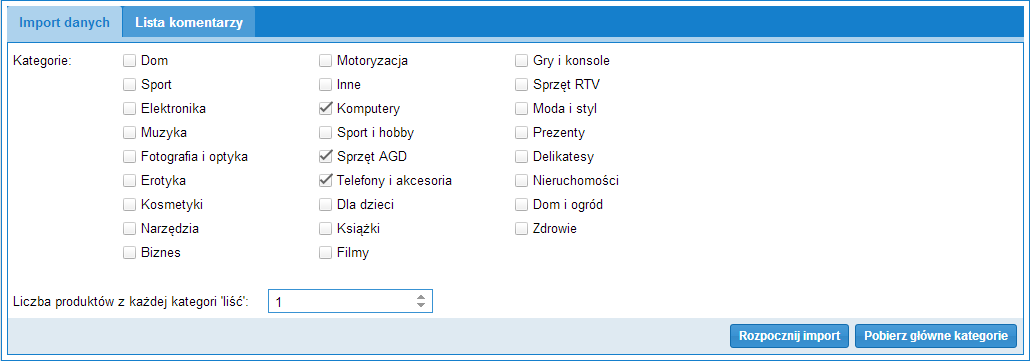
\includegraphics[width=1.00\textwidth]{images/Import.PNG}
	\caption{Widok panelu imprtu danych.}
\end{figure}

Przy pomocy przycisku „Pobierz główne kategorie” Użytkownik ma możliwość importu głównych kategorii. Kategorie główne, są to kategorie, które nie mają kategorii nadrzędnych. Po wykonaniu tej operacji, możemy wykonać właściwy import, wybierając interesujące nas kategorie oraz wciskając przycisk „Rozpocznij import”.\linebreak 
Import polega on na pobraniu wszystkich kategorii potomnych w~ramach wybranej kategorii oraz produktów należących do kategorii znajdujących się na samym dole hierarchii.
